\chapter{Serverless computing}

\section{Origins}

The growth of cloud computing significantly influenced the way how server management and server application development are perceived. Around fifteen years ago, most of the companies were entirely responsible for managing their software, altogether with the hardware and infrastructure it was running on \cite{RobertsChapin2017}. Around that time, first services capable of outsourcing some part of infrastructure overhead emerged, which started the idea of cloud computing.

Amazon Web Services was one of the first service providers that enabled companies to rent computing capacity by announcing the launch of Elastic Compute Cloud (EC2) in August 2006. It was the first Infrastructure as a Service (IaaS) product on the market that allowed companies to run their server applications on Amazon's machines that are billed per usage time and are available within minutes from requesting new resources.

Leveraging such a service model brings a handful of benefits. It reduces the labour cost by outsourcing hardware management to the provider and infrastructure cost by paying based on actual usage of services. Furthermore, it enables companies to scale the number and type of servers in correlation with the traffic and demand for processing. Finally, it encourages testing new solutions developed by companies by decreasing the lead time, by making the required infrastructure available within minutes instead of months, utilising favourable billing flexibility.

The cost of IaaS solutions is profitable to providers, because of technical improvements done in terms of hardware virtualization and the economy of scale on which they operate. Shortly after other vendors such as Microsoft, Google and DigitalOcean embraced the notion of public cloud by providing services and resources from their own data centers. At the same time, tools like Open Stack enabled companies to use hardware from their own data centers in the same way, forming the idea of private cloud.

The next step in the cloud evolution is Platform as a Service (PaaS). As a layer on top of IaaS, it adds operating system to the outsourced infrastructure stack enabling to deploy the application code directly. In that model, the platform takes responsibility for managing the operating system as well as monitoring and running the application. Google App Engine, AWS Elastic Beanstalk and Heroku platform can be distinguished as most popular PaaS solutions, while one of the most frequently mentioned self-hosted variant is Cloud Foundry.

The growth of containerisation technologies introduced another type of service called Container as a Service. Technologies like Docker allowed developers and system administrators to deliberate more clearly on the application requirements and separate it from the operating system. Solutions such as Marathon running on top of Mesos and Kubernetes introduced a possibility to manage and orchestrate containers on self-hosted machines. The services provided by cloud vendors include for example Google's Compute Engine or Amazon's Elastic Container Service (ECS) or AWS Fargate. With the growing popularity of Kubernetes, dedicated services leveraging that platform such as Amazon Elastic Kubernetes Service (EKS) and Google Kubernetes Engine (GKE) emerged.

Each of the described services are next generations of infrastructure outsourcing, which raise the level of abstraction from the development perspective and hand off more and more responsibility related to infrastructure management to the cloud vendor. Despite the fact, for each of the mentioned services the smallest unit of processing is some sort of server application or running application process in the virtual machine or within the container.

Serverless is considered as a next step in the cloud computing progression. The term serverless was one of the first used by Ken Fromm in his paper \cite{KenFromm}. It describes the notion of architecture migration from monolithic applications running on servers into distributed systems that consist of multiple components, processes and data stores with the goal to perform various tasks and process numerous flows. The serverless architecture enables developers to make a mindshift accordingly. Computing resources can be used as services, which makes it possible to shift thinking from the servers level to the tasks level, taking away the complexity of infrastructure management. The servers are still used underneath, but developers don't need to worry about managing them any longer.

Such an architecture model was leveraged firstly by mobile applications built on top of hosted database solutions such as Parse (later acquired by Facebook) and Firebase around 2012 (obtained by Google). Nonetheless, the most significant event shaping the serverless architecture was the announcement of AWS Lambda in 2014, altogether with the introduction of API Gateway in 2015. By the middle of 2016, major cloud vendors such as Microsoft and Google embraced the serverless architecture approach and started offering their services for developing serverless applications.

\section{Defining serverless}

Despite the fact that the idea of serverless computing emerged about a decade ago, it has been already widely adopted by leading cloud providers. Currently it covers a range of technologies, components and cloud services. Nevertheless, there is no clear and concise view on what ''serverless'' is. Various vendors, organisations and research groups tried to define what the serverless term means for them.

Cloud Native Computing Foundation of the organization working towards standardisation of numerous cloud-related technologies and components. It maintains a sustainable ecosystem for cloud native software by bringing together and collaborating with various members of the cloud community. According to ''CNCF Serverless Whitepaper'' \cite{CNCFServerless}.

\begin{quotation}
Serverless computing refers to the concept of building and running applications that do not require server management. It describes a finer-grained deployment model where applications, bundled as one or more functions, are uploaded to a platform and then executed, scaled, and billed in response to the exact demand needed at the moment.
\end{quotation}

Another definition considering the serverless service capabilities can be found in a booklet made by Mike Roberts and John Chapin titled ''What is Serverless?'' \cite{RobertsChapin2017}.

\begin{quotation}
\noindent A Serverless service:
\begin{itemize}
    \item Does not require managing a long-lived host or application instance
    \item Self auto-scales and auto-provisions, dependent on load
    \item Has costs that are based on precise usage, up from and down to zero usage
    \item Has performance capabilities defined in terms other than host size/count
    \item Has implicit high availability
\end{itemize}
\end{quotation}

The cited definitions contain insightful information about features of serverless architecture and capabilities of its components. These can be summarized as follows:

\begin{itemize}
    \item Serverless architecture defines the new model of developing and executing workloads. The application consists of multiple serverless components configured together to run the business logic within the application code, designed to be executed in a serverless environment.
    \item It does not require to maintain, provision and monitor servers and applications. Serverless does not mean that there are no servers - the overhead of managing them is handed off to the cloud provider.
    \item Deployment model is more granular. Having the application built from multiple components configured to work together, the deployment can update only selected ones.
    \item Platform is responsible for provisioning and executing the applications. With a large resource pool maintained by cloud provider and the possibility to quickly allocate it, the solution can be scaled automatically to the current load requirement almost instantly.
    \item The cost is proportional to the resource usage. Each of the components involved in performing the computation is billed granularly, with an accuracy to hundreds of milliseconds or number of executed operations, with no cost when being idle. Executing hundred operations in parallel will cost the same amount of money as running that workload sequentially.
    \item The performance is not related to the host size. Some of the cloud providers enable customers to choose how much memory and CPU can be allocated for the environment. Nevertheless, the configuration is abstracted from the capabilities of the underlying machine that is used as an application execution environment.
    \item The serverless components are built with high-availability and fault-tolerance in mind. Despite the fact that developers are no longer concerned with servers, the underlying vendor's machines can still fail. When using serverless services we expect that cloud vendors will provide transparent high availability for its services. Although, as developers it may be necessary to handle some errors and failure occurrences properly.
\end{itemize}

\section{Serverless components}

When considering the serverless architecture we refer to a range of technologies provided by cloud platforms. Two different areas can be distinguished, defining two distinctive components:

\begin{itemize}
    \item \textbf{Backend as a Service} refers to third-party services or generic components capable of replacing some part of a server side application, that has been previously developed internally or self-provisioned. It exposes an API which allows for integrating the component with the rest of the application.
    \item \textbf{Function as a Service} is an event-driven execution environment for running application code within stateless and ephemeral containers with strictly limited execution time.
\end{itemize}

Aforementioned components used simultaneously enable developers to build fully-fledged solutions utilising serverless architecture and are offered together within a single cloud platform.

Even though presented areas serve different roles, they share common features and capabilities. These could be listed as follows:

\begin{itemize}
    \item Require no resource management and are entirely provisioned by cloud provider
    \item Billing is proportional to actual usage
    \item Utilise the event-driven model for processing
    \item Underlying platform ensures automatic horizontal scaling, high availability and fault tolerance
\end{itemize}

\subsection{Backend as a Service}

The concept of Backend as a Service (BaaS) gathers various domain-generic, repeatable application components capable of replacing some part of application logic or providing some functionality. They can be accessed and integrated into developed applications through API defined by its provider.

Taking into consideration most popular requirements of various applications, the majority of them need to store and manage the data. Depending on the requirements the information should be stored in a structural way in databases or can be stored regardless of their shape in file storage service. For teams developing mobile or web applications it is convenient to rely on some third-party service to store and access the data directly from the application. Services like Google's Firebase meet such requirements and give access to the database entirely managed by a cloud vendor. Depending on the complexity of developed product it may be required to incorporate some more advanced components to process required tasks or flows reflecting the business logic of application. Mechanism serving as notification services, exposing some publish-subscribe capabilities for defined events could be applicable in that case. It is essential to notice that such components are replacing previously self-hosted components such as databases or other data stores, message-brokers or other services responsible for processing data streams incoming from various sources.

Looking closer from the application logic point of view, there are also repeatable functionalities implementations that can be extracted and reused across multiple developed applications. Most of the products will require some features enabling users to manage their identity and associated permissions. Most of the time, the capabilities will be not only limited to registering and logging users, but it will also include integrations with other services as identity providers. Managing and sending emails can be considered as another functionality that can be extracted into separate component from the code perspective and reused in other applications. Products such as Auth0 (serving as fully featured authorization and user management service) or Mailgun (capable of managing and processing emails) makes it possible to replace entirely the repeatable part of business logic.

% TODO:rb update chapter reference
Specific components and services that can be classified as Backend as a Services will be covered in more details in chapter ... when analysing services provided by leading cloud vendors. All of the mentioned components enable developers to create fully fledged applications and services similar to the solutions built using self-hosted component equivalents. The difference is that mentioned components are characterized by capabilities of the serverless architecture. They are provided by cloud vendors, who take responsibility for managing, provisioning and scaling them depending on the demand. Moreover, the possibility to replace the repeatable application features by utilising third-party services enables developers to iterate faster and shorten the lead time.

\subsection{Function as a Service}

The second area refers to Function as a Service (FaaS) that serves as an environment for executing application code. It introduces a new architectural approach in terms of developing, structuring and deploying the application logic, which is oriented towards individual tasks and operations.

Mike Roberts briefly described the idea of FaaS \cite{MartinFowlerServerless} based on the definition of AWS Lambda \cite{AWSLambda}, which is currently one of the most commonly used implementation of a Function as a Service platform. Based on his summary several main features of FaaS can be highlighted:

\begin{itemize}
    \item The main idea of FaaS is to run application code without managing servers and application processes. It is a common feature with other approaches like CaaS or PaaS, where the responsibility for managing applications is placed on the cloud vendor. However, the key difference with FaaS is the fact that the function execution time is strictly limited in contrast to long-lived processes existing in aforementioned services.
    \item The functions are invoked and executed on the underlying platform in response to specific events occurring or incoming into the system. Based on that cloud provider handles resource allocation and runs the function code in an ephemeral container, created based on runtime needs. These are destroyed shortly after the event is processed by the application logic in the function. Together with limited execution time it is a significant architectural restriction for the FaaS model.
    \item Given the fine-grained execution model, horizontal scaling can be easily and automatically handled by the cloud provider. When there is an increased traffic in the system, the platform responsible for executing functions allocates resources to create and run more functions, which will be capable of processing the increased traffic. An analogous situation takes place when there is no traffic, therefore there is no need to allocate resources for running functions code.
    \item As a consequence of greater granularity of application code and managing the function execution by cloud provider, the deployment process differs from the traditional system. Each function can be independently packed and uploaded to the FaaS platform, which takes responsibility for executing it.
    \item Most of the cloud platforms do not require to use neither predefined framework nor programming languages. Although cloud providers define the list of environments and languages that are supported by the platform, any process that is bundled into the artifact and can be executed from it is capable of processing the incoming event.
\end{itemize}

Selected aspects of Function as a Service architecture are covered in more details based on ''CNCF Serverless'' whitepaper \cite{CNCFServerless} in the following sections.

\subsubsection*{Function lifecycle}

Before analyzing the execution model in more details, it is important to examine the deployment process accompanying the development of a function. Alongside with providing the function code, the developer is responsible for specifying one or more events upon which function will be triggered. Additionally, metadata defining for example the function version, environmental variables, execution role and other configuration parameters can be defined. The function and specification prepared in that way is uploaded to the cloud provider and processed by a dedicated builder entity, resulting with a function artifact (depending on the cloud platform and selected runtime it can be a binary file, container image or a package). Next, it is deployed on a cluster managed by a FaaS controller responsible for provisioning, controlling and monitoring function instances based on incoming events.

\begin{figure}[h]
    \centering
    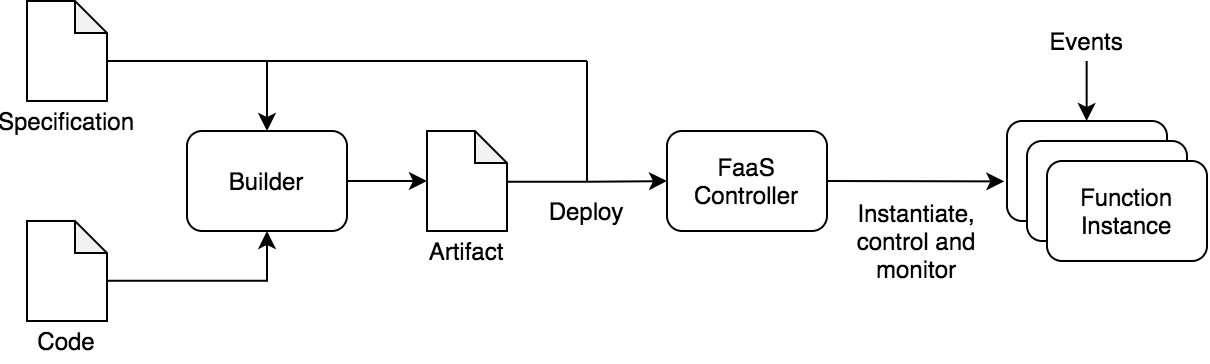
\includegraphics[width=0.8\textwidth]{assets/02-serverless/ServerlessDeployment.png}
    \caption{Function deployment and invocation process}
    \label{fig:cloudguru-architecture-diagram}
\end{figure}

Furthermore, the serverless platform may provide additional actions related to function management such as executing, publishing, updating and deleting the function or its metadata. Also, a particular version of the function can be labeled or aliased, which can come in handy when operating the serverless system on a larger scale. Logs and statistics are gathered alongside function execution.

The function is executed in an event-driven model and within strictly limited duration. The whole process begins when an event triggering a particular function is dispatched. It is detected and registered by an underlying serverless platform. The controller responsible for managing function execution looks for functions associated with incoming events, gets its code and configuration and allocates an adequate amount of resources from the managed resource pool. The new execution environment is created inside a lightweight, ephemeral container and language runtime for the function is bootstrapped. When it's ready, the triggering event is redirected and processed by the application logic contained in the function code.

The results of computing are sent back to the event dispatcher. Other, newly created events can be dispatched during function execution. The computing duration is limited by the majority of service providers up to a few minutes, after that the computation is completed with timeout. At the end the lightweight container containing the execution environment is destroyed.

Most of the providers delay the container deletion for longer than a couple of minutes due to optimisation related with reusing the same container instance when the next event occurs in the system. Reusing an already initialised execution environment is called a ''warm start'' and allows to reduce the startup latency related to resource allocation and runtime preparation. The opposite situation takes place when the new container instance needs to be initialised and the host process needs to be created. Most of the time it requires additional time impacting the request processing duration - it is called ''cold start''.

\begin{figure}[h]
    \centering
    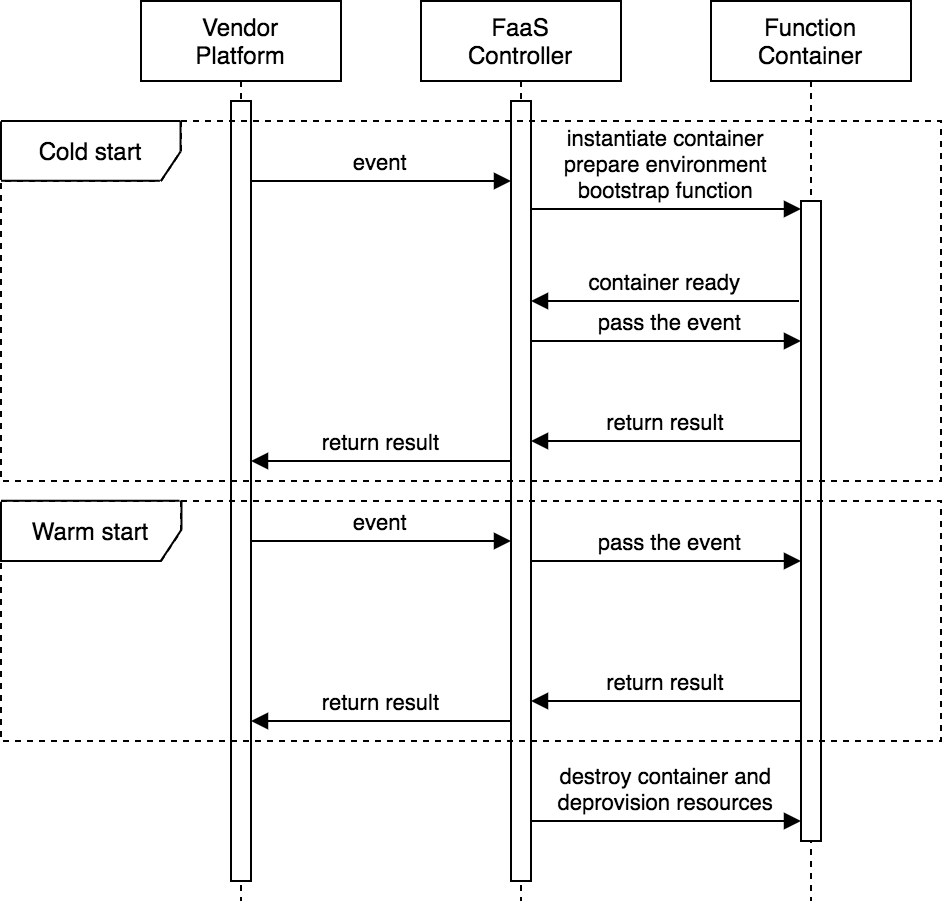
\includegraphics[width=0.7\textwidth]{assets/02-serverless/ServerlessExecution.png}
    \caption{Function execution process considering ''cold start'' and ''warm start''}
    \label{fig:cloudguru-architecture-diagram}
\end{figure}


\subsubsection*{Function environment}

The characteristic of the function environment has been already drafted during description of the function lifecycle. Due to improvements in the software virtualisation area, cloud vendors can benefit from efficient and elastic management of large resource pools. It enables vendors to allocate efficiently lightweight and ephemeral containers, serving as an execution environment. Each of them is initialised to execute code of one of the functions at a time and it is destroyed shortly after, releasing the resources to the common pool. Even though containers can be reused for the optimisation purposes when handling subsequent events occuring in the system, it is not guaranteed by the serverless platform and should not be taken for granted by developers, that some data could be preserved for subsequent invocation.

Such an architecture leveraging stateless containers allows for automatic horizontal scaling. When multiple concurrent events occur within the system, the platform is capable of creating a separate container to process each of them independently. In order to handle spikes of traffic effectively, quick provisioning of the containers and reducing their startup latency is required and it is a purpose many research works and improvements made by both researchers and cloud vendors

As mentioned before, ephemeral containers are dismissed shortly after the execution alongside with their internal state. For some types of computing it would be desirable to preserve that state. To address that issue, external components need to be introduced to persist the data. Nevertheless, it introduces the need to communicate with some external service and it is often associated with additional delays resulting from the communication overhead.

\subsubsection*{Function invocation}

The serverless architecture utilises an event-driven processing model. The developer's task is to define configuration that maps events coming to the system with appropriate functions. Each of dispatched events can trigger one or more functions as well as each function can be invoked by one or more predefined events - there is a many-to-many association between function and event sources. The mapping can also refer to a particular version of the function or alias, which can greatly simplify the deployment process by replacing the function code for a given alias without modifying the configuration.

Various data sources can be divided into several categories among which we can distinguish:

\begin{itemize}
    \item Endpoint Services - Most of the time associated with API Gateway components, which introduces mapping between request coming from APIs, such as REST or Websocket and associate them with corresponding functions
    \item Storage Services - Category includes numerous BaaS components provided by a cloud vendor like databases, file storage or cache services. Events can be emitted based on operations performed on the data such as creation, deletion or modification of it.
    \item Messaging Services - Services providing mechanisms for data streaming, message brokers or various services sending notifications.
    \item Scheduled events - That category include services capable of emitting events periodically at a given time or at a selected interval
\end{itemize}

Based on the use case, several invocation types can be differentiated:

\begin{itemize}
    \item Synchronous Request - Includes cases when the client sends a request and waits for the response. It is used most frequently for HTTP requests.
    \item Asynchronous Message Queue Requests - Refers to events emitted from various data sources when messages are published to some exchange that later distributes it to other subscribers. Messages are delivered exactly once without strict ordering.
    \item Event Streams - Are based on streams of messages, logs or files. Sequence of record is most of the time partitioned into several shards.
    \item Batch Jobs - Refers to jobs that can be splitted into smaller tasks and processed in parallel by multiple functions. The entire process is completed when all subsequent tasks are finished.
\end{itemize}

\section{Benefits and challenges}

The emergence of serverless architecture has met with great interest from various software architects, developers and companies that noticed numerous advantages of the serverless architecture. In addition to the promise of significant cost reduction, the development and operational opportunities and reducing time to market are just a few of the benefits that serverless introduces.

Nevertheless, serverless architecture also has many disadvantages inherently connected with its nature. Some of them have been addressed by various cloud vendors working towards improving their services and mitigating the problems. Despite the fact that many companies already adapted it, the technology is still not fully mature. There is much research ongoing in the various areas conducted by both researchers and cloud providers.

Among the many reports and articles discussing the advantages and drawbacks connected with the serverless architecture \cite{MartinFowlerServerless} \cite{BerkeleyServerless} \cite{ServerlessComputingSurveyOfOpportunitiesChallengesApplications} \cite{LeveragingServerlessCloudComputingArchitectures} has been selected. Based on the conclusions included in the papers, listing of benefits and challenges of the serverless architecture has been created, dividing the latter into three distinctive categories.

\subsection{Benefits}

\subsubsection*{Reduced development and operational cost}

Serverless is essentially another step in the process of infrastructure management outsourcing similar to IaaS and PaaS. Instead of requesting resources, developers can provide an artifact including code to be executed and the cloud platform is responsible for provisioning the resources and executing the code based on defined triggers configuration. The responsibility of managing the servers, databases and application execution is transferred to the cloud provider \cite{BerkeleyServerless}. The favourable and competitive prices are available due to economy of scale in which one vendor is running thousands of predefined services, effectively sharing the infrastructure among the customers.

The labour cost connected with the serverless architecture is also reduced, because there is less work related to managing the serverless solution compared to the self-hosted alternative. There is no need to setup, maintain hardware and restore it to proper condition in case of failures - new resources can be allocated and be ready to work with, within a moment from requesting it. The development cost is also reduced due to frequent usage of BaaS components replacing the application elements that were previously developed in-house, now can be incorporated with the application logic. An example of such approach is aforementioned Auth0 providing the authentication capabilities or Firebase enabling client applications to directly communicate with server-side databases, accordingly providing proven authentication mechanisms for different types of users and removing much of the database administration overhead \cite{MartinFowlerServerless}.

\subsubsection*{Autoscaling with proportional cost}

The serverless billing model refers to paying proportionally to the time resources are used instead of calculating the cost based on the size of cloud resources as in IaaS or PaaS offerings. By tracking the load with a greater fidelity, scaling up quickly in case of increased demand and scaling down in the absence of it, customers are actually charged for the time the code was executed rather than the resources used to execute their software \cite{BerkeleyServerless}.

Additionally with the greater granularity, only the components affected by increased demand can be scaled accordingly compared to the conventional serverful computing. The serverless processing is characterized by the instant horizontal scaling, which is an ability to parallelize heavy workloads almost instantly on demand and deprovisioning resources shortly after, that is an automatic process handled entirely by the cloud provider. It enables companies to shift from the capital expense to the operational expenses when running their software, which removes the need to invest beforehand in costly hardware before the application or service is created and deployed \cite{LeveragingServerlessCloudComputingArchitectures}.

The cost reduction is most visible when the service has to process the occasional or inconsistent traffic. In the first case the processing will be executed based on the event, billed accordingly to execution time and not paying for idle, which is significantly more efficient compared to the self-hosted solution in which some server is running the application all the time. When running the application in the second case, it may be necessary to have enough hardware to handle the highest demand to ensure the running service is capable of handling all the requests. With the serverless solution the cloud provider is responsible for scaling to handle the demand. The customers pay only for the additional time hardware was computing to satisfy the higher traffic. Comparing to provisioning virtual machines there is no risk of overprovisioning (when demand is handled on time, but the resources are not fully utilised) or underprovisioning (when the average processing capacity is optimised, but the highest traffic may not be handled on time or even not at all). These examples are deliberately picked to showcase the significant cost savings of serverless, but on the other hand when the traffic shape is making a good utilisation of running servers, the cost of using serverless technologies can be higher. Lastly considering the serverless model, any performance optimisations making the function execution shorter or reducing the number of requests to some other BaaS component can accordingly reduce the cost \cite{MartinFowlerServerless}.

\subsubsection*{Easier operational management}

Considering the scaling is automatically handled by the cloud vendor, there is no need to hire qualified administrators to manage and scale the application and make sure that the service is running properly, which leads to further cost reduction. The packing and deployment process for serverless solutions is also simplified compared to deployment of new versions of software to the servers. There is no need to manage some scripts or specified software responsible for managing the deployment, the serverless solution can be packed, zipped with appropriate configuration and deployed to the cloud, where the cloud vendor handles the rest of the process. In the fully serverless solutions the system administration role can be effectively minimised by the serverless platform when embracing the proper process automation \cite{MartinFowlerServerless}.

\subsubsection*{Development opportunities}

Serverless solution is appealing, because of the possibility to reduce the cycle time. The focus of development can be put on the business logic and developing the product instead of managing the infrastructure.

The serverless architecture brings new architectural opportunities and provides some interesting architectural properties. For example the automatic horizontal scaling brings yet another benefit - the software architects and developers no longer need to think about designing the solution to ensure the scalability, cause it is provided out of the box by the cloud platform. Similar situation can be noticed for the implicit failover. There is no need to run another instance to pick up the computation once the first one fails. FaaS handles implicit failover by retrying the execution on newly provisioned functions once the initial on crash \cite{LeveragingServerlessCloudComputingArchitectures}.

The cloud platform provides various BaaS components, giving a possibility to incorporate and integrate them with the developed solution. They are giving various capabilities not only related with authentication, storing data or exchanging messages in a publish-subscribe manner, but also give some more sophisticated services including documents and image processing, generating transcriptions or incorporating machine learning for advanced prediction. It gives the opportunities for developers to look at a vast area of new possibilities with a matter of integration and configuration of some of the services.

It is especially beneficial for agile teams gearing towards lean and agile processes, by reducing time to market, which is understood as the time from an idea until the product is available for the customers. Having the better granularity of code and without the need to manage the infrastructure, the new version of a service can be released more frequently, moving towards the idea of continuous deployment. Along with the granular billing model the companies can try out new solutions with minimal cost and friction. The new experiments can be deployed within a moment since the development is completed, enabling the product owners to set the mindset of continuous experimentation. The proof of concept feature with the limited traffic will cost proportionally low or could be even free if the resource utilisation fit into the free tier provided by some of the cloud providers \cite{MartinFowlerServerless}.

\subsubsection*{Greener computing}

The growth of awareness about environmental problems has influenced the way the data centers are built. To fulfill their energy requirements cloud providers host their data centers near the renewable energy sources to reduce the fossil-fuel emission. Contrary to the typical data centers, which are delivering only some percent of their real computing output, while some of the servers can be running idle inefficiently consuming the energy.

Cloud infrastructure partially mitigates that problem, because the companies are renting the computing resources based on the demand, rather than provisioning the servers on their own, especially when these are run without adequate awareness about the capacity management. When using IaaS, PaaS or self-hosted solutions most frequently the users are responsible for scaling the services, preferably overprovisioning the resources which leads  to inefficient energy utilisation. The cloud provider takes the responsibility for the serverless solutions by provisioning the compute resources and handling the capacity decisions to fulfill the needs, leading to far more efficient resource and energy utilisation across data centers and reducing the environmental impact \cite{MartinFowlerServerless}.

\subsection{Challenges related to the nature of serverless architecture}

\subsubsection*{Function state management}

As mentioned before the FaaS are effectively stateless and due to that have a significant limitation when it comes to the local state. It should be assumed that the state from one invocation will not be available in another invocation of the same function, which is connected with the lack of control over the ephemeral container function is running in. To share state between subsequent function execution it should be preserved in some external component like database, cache or external object storage, which introduces significant communication overhead leading to latency increase \cite{MartinFowlerServerless}.

It highlights that some types of computation relying heavily on fine-grained state sharing may not be suitable for the serverless model. Two distinctive types of storage needs to be addressed. First of them is a low-latency ephemeral storage enabling to transfer data between functions and maintain the application state during application lifetime. Once processing is finished, the state can be discarded. To achieve that some in-memory cache with optimised network and low latency operations can be considered. Nevertheless, the main challenge there is to provide automatic scaling, allocating and freeing resources and ensure access protection together with performance isolation. The second type refers to durable storage, as a long-term data storage with mutable semantics of a file system. It should also be transparently provisioned, ensure proper level of isolation, security and performance predictability, but contrary to ephemeral storage the data should be durable and the removal should be explicit along with maintaining low cost \cite{BerkeleyServerless}.

\subsubsection*{Function communication and data transfer}

The service built using the serverless architecture is essentially a composition of many functions and BaaS components working together to provide the desired functionality. To achieve that, functions need to communicate somehow  and exchange the data. In other cloud services communication can be attained through network addressing, but in serverless architecture functions are ephemeral and anonymous. The function-level addressing is not available and they need to communicate through intermediate storage or messaging service introducing additional latency and which can be pretty expensive with finer-grained communication patterns. Additionally, the fact that functions can be allocated and load balanced according to the current utilisation of resources in the data center impacts the performance when the data needs to be transferred to the function. Due to that the data caching in a serverless environment can be more difficult to be implemented in an effective way since the functions are placed and executed independently \cite{ServerlessComputingSurveyOfOpportunitiesChallengesApplications}.

Some of the communication patterns known from machine learning or big-data analysis software like broadcast or aggregation require sending more messages and can be less performant when implemented in a serverless architecture. Compared to the software running on virtual machines the tasks can share a copy of the received data and perform local aggregation to limit the message overhead and amount of data being sent. Moreover, the serverless component utilises most frequently some intermediate component working in a producer-consumer pattern to send the data, which introduces additional communication delay. Due to lack of addressability the functions are unable to communicate directly, for example calling one another when the data is present or coordinate some distributed operation \cite{BerkeleyServerless}.

To address that problem cloud providers could enable developers to assign the group of functions to the same machine instance, reducing the data exchange overhead or compute the communication graph to place functions efficiently, but it would reduce the flexibility of cloud providers and data centers utilisation. Some of the offerings such as AWS Step Function or Azure Durable Functions try to address the function orchestration problem, by running a sequence of lambda functions as event-driven workflow and efficiently maintain the application state between the subsequent invocations.

Some of the approaches of various practitioners consider some sort of hybrid solution to address the problem of externalized state constraint and lack of function addressability. The low-latency application can be run as regular, long-running servers handling the requests and keeping the context in local memory, handing off the fully contextualized requests to FaaS executed concurrently to process some computation without need to lookup for external data.

\subsection{Cloud platform and vendors challenges}

\subsubsection*{Vendor dependency}

As with any outsourcing technology some control of the system is given up to the service provider and it is no difference with the serverless. The cloud vendor can put some constraints on how the clients use their services in form of unexpected limits or API changes to be more likely to deliver the reliability on its side. Similarly when using BaaS components, developers no longer need to implement and maintain them, but it is not guaranteed that the external services will be running without some issues or unexpected failures. If the cloud platform would satisfy the needs of hundreds of customers or the smaller group, it will most probably choose the majority to ensure accountability of services \cite{MartinFowlerServerless}.

\subsubsection*{Vendor lock-in}

The cloud provider selection is a significant decision when building some service using the serverless architecture not only due to their offerings, but also due to differences in their services implementation that makes the further shift harder or even almost impossible without major changes. When taking a closer look at the function invocation semantics, each of them depicts the different interface and events triggering it. The divergence also occurs on the level of BaaS components which expose various behaviours and API which may even require to change the architecture solution in some cases. Moreover, operational tools related with deployment, logging, monitoring and configuration management will most probably differ and require migration.

When migrating the serverless solution from one of the cloud providers to another one, some parts of the system can be translated more easily, but others can have a significant impact on the whole architecture of the developed solution. For example porting of some function code between cloud platforms won't be possible without migrating other chunks of the architecture. Some companies adopt multi-cloud approaches leading to developing and operating the application in a way that is agnostic to the cloud vendor. Most frequently it is a more costly solution, which makes it impossible to apply benefits, optimisations and more specialised components provided by the cloud vendor \cite{MartinFowlerServerless}.

\subsubsection*{Startup latency and platform improvements}

Serverless functions have much lower startup latency than the application executed on the virtual machines, but because of the frequency of using new function instances the low startup time is crucial to provide efficient processing. The function startup time consists of scheduling and allocating the resources to run the function, establishing the environment for code execution and initialising the libraries and data structure to run the function code.

When the function is executed for the first time after a longer period of inactivity or when a new version is deployed, the function bootstrapping process will consist of all of the steps forming aforementioned "cold start". Providers already noticed that resources and environment of the function containers can be reused to save some of the bootstrap time. Nevertheless, the most noticeable latency related to the full function setup has a significant impact on the service performance from the user point of view \cite{BerkeleyServerless}.

Different approaches are currently available to mitigate that problem, but they are coming with an additional cost. The serverful instances can handle low-latency applications well, because they are always running and ready to serve the traffic. Similarly, function can be pre-warmed regularly to ensure the resources and environment is ready to satisfy the incoming request. AWS Provisioned Concurrency is one of the dedicated extensions to the AWS Lambda service, while Serverless Framework includes some plugin enabling that by registering scheduled events that keep functions warm.

Another factor limiting the serverless function execution is constrained execution duration. Various FaaS offerings from the biggest cloud providers limit the execution time to elastically manage their resource pool. Beyond that cloud vendors could increase the transparency of services and provide more clear expectations towards their platforms to increase the degree on which customers can rely on them \cite{MartinFowlerServerless}.

\subsubsection*{Multitenancy problem}

To achieve efficient resource utilisation multiple cloud functions from different applications and customers are executed on the same virtual machine enabling the cloud platform to provide affordable services. Cloud vendors are doing their best to provide a proper level of isolation between different tenants and application execution. Most of the biggest providers developed mature technology to ensure the high quality of their services, but for other less mature solutions some problems can be noticeable. Among the most common issues with robustness (error in customer’s software causes failures of other), performance (one customer takes majority of the machine resources causing others to slow down) or even security (seeing data of other customers) can be distinguished \cite{MartinFowlerServerless}.

\subsubsection*{Security concerns}

Serverless architecture opens a large number of security questions taking into consideration the attacks surface of serverless composition which is not fully researched yet. On one hand the cloud providers should ensure proper security level of their services with monitoring the services and patching eventual vulnerabilities, but on the other hand executing the computation within a shared resource pool extends the area of potential attacks when breaking out from the ephemeral function container \cite{LeveragingServerlessCloudComputingArchitectures}.

To address that problem, different tenants and applications could be physically isolated, but it can impact the resource allocation and the startup time optimisation. The greatest challenge is to provide a proper function level sandboxing while maintaining the short startup time enabling a shared environment between repeated function invocations. It could be possible by snapshotting the instance locally or using lightweight virtualisation technologies and it is a subject of active research and improvements \cite{BerkeleyServerless}.

Another security concern takes into account the direct access to the services directly from the client applications, which requires additional care, cause there is no protection of the server application available in serverfull applications. Utilising various services from different providers makes the area of potential vulnerabilities larger and establishes multiple possible ways to breach into the system. The communication between them needs to be properly integrated and protected.

When building some service utilising different functions and components it will require cooperation between them to perform the processing. Each of the functions should have granular access policies granting only the required permissions to the BaaS components used by the function. Maintaining and validating the security and access policies is not a trivial task, especially when the service and number of its components and access pattern are increasing overtime \cite{MartinFowlerServerless}.

\subsection{Development and operational challenges}

\subsubsection*{Development and debugging}

The serverless computing introduces a relatively new approach for developing services and with lack of knowledge and proper modeling paradigm it can lead to many development approaches that can reduce the quality of service and complicate the collaboration between developers. New ideas and patterns are created and researched to utilise serverless architecture effectively, which leads to high demand for practitioners and architects aware of the best practices and providing reference architectures \cite{ServerlessComputingSurveyOfOpportunitiesChallengesApplications}.

Developing the fully serverless solution introduces additional difficulties due to inability to replicate the cloud environment locally. Some of the cloud vendors provide tooling to execute the functions locally, for example AWS Serverless Application Model enables to execute functions locally and pass the event payload saved beforehand. Altogether with the execution, some tools enable function debugging, while Azure even makes it possible to run local debugging for functions triggered by remote events. Nevertheless, to verify behaviour of other services it is essential to deploy the service and verify it's behaviour in a cloud environment. The idea of distributed monitoring, which enables tracing the flow of a single request across multiple components, is covered by services such as Amazon X-Ray and other third party offerings.

Over the recent years the ecosystem of serverless tooling significantly evolved providing various products and services which helps with the development and operational aspects of managing serverless applications and services. The process of deployment and bundling improved with the introduction of Serverless Framework, AWS SAM and AWS Cloud Development Kit, which allow to define the architecture using many popular programming languages. Lastly, the serverless tooling helps with operational aspects enabling various higher level releases approach, supporting traffic shifting, A/B testing, blue-green deployments or canary releases which are essential when releasing complex, distributed application that consist of hundreds of functions \cite{MartinFowlerServerless}.

\subsubsection*{Testing}

The unit testing of serverless functions, which are initially pure functions that are mapping input to the output, is fairly simple. Contrary to the integration testing, because most functions use various BaaS components or other external services creating a dependency in tests. Some of the vendors supply mocked implementations or stubs that can be  incorporated into tests and imitate the BaaS behaviour. Nevertheless, the idea giving the most confidence is to deploy the service into the cloud environment and conduct some end-to-end tests to verify the quality of software.

The ideal and most appealing approach would be to create a suite of automated integration tests, deploying the functions and infrastructure configuration to the cloud as part of the integration pipeline to verify if it is working as intended. However, running such tests creates additional cost with every execution, due to resource usage for processing the test data. It may also require more work compared to writing integration tests for regular services created as stateful applications. 

One radical change that could be embraced is the idea of testing in production and monitoring-driven development, that is related to switching subset of the traffic to the newer version and comparing the observed behaviour with the previous one \cite{MartinFowlerServerless}.

\subsubsection*{Monitoring and observability}

Monitoring the service created by utilising the serverless architecture can be harder due to the ephemeral, granular and distributed nature of processing. Aforementioned distributed monitoring is especially desired to trace the flow of a request not only to verify if the application works correctly, but also to give more insight into performance aspects directly correlated with the cost \cite{LeveragingServerlessCloudComputingArchitectures}.

Most cloud vendors provide some tooling to monitor the system and there are many third party offerings helping with achieving better observability in that area. Despite the fact that more of the operational context related with infrastructure management is handed off to the cloud vendor, there is still plenty of administration work with ensuring monitoring, proper security level and verifying that the appearance of alarms when crossing some of the established limits, does not affect the proper service execution. Introducing various checks in the deployment process can ensure that the service quality is preserved. Techniques like preemptive load testing and chaos engineering can help simulate various critical situations and verify that the system is able to cope with them \cite{MartinFowlerServerless}.

\section{Cloud providers}

\subsection{Providers Overview}

\subsubsection*{AWS}

\subsubsection*{Azure}

\subsubsection*{GCP}

\subsubsection*{Other providers}

\textbf{IBM}

\textbf{Oracle}

\textbf{Alibaba}

\textbf{Netlify}

\textbf{Vercel}

\textbf{Cloudflare}

\subsection{Open Source}

% https://arxiv.org/pdf/1911.07449.pdf

\subsection{Differences between providers}

% - available services, 
% - approaches to develop serverless apps, 
% - can Open Source replace providers?
% - table comparison ???

\section{Use cases}

% https://pages.awscloud.com/rs/112-TZM-766/images/Asset2-optimizing-enterprise-economics-serverless-architectures.pdf - examples
% https://www.simform.com/serverless-aws-lambda-examples/
% https://dashbird.io/blog/companies-using-serverless-in-production/
% https://dashbird.io/blog/serverless-case-study-coca-cola/, https://aws.amazon.com/solutions/case-studies/coca-cola-freestyle/

% \cite{ServerlessArchitectureOnAWS}
% - suitable for some types of processing - reference to benefits
% - serverless is suitable for building whole systems, create isolated components or implement specific and granular tasks - serverless can be applied to small and large tasks
% - serverless is not only about processing by lambdas, but also 3rd party services, which amke possible to cut down the work

\subsection*{Application backend}

% https://livebook.manning.com/book/serverless-architectures-on-aws/chapter-2/36 - CloudGuru

Serverless technologies are an appropriate solution for building scalable application backends for all kinds of web, mobile and desktop applications. They are favorable for this use-case, because the infrastructure management can be effectively automated ensuring dynamic scaling to meet uneven demand, while ensuring granular and predictable billing. Despite the fact that serverless technologies are a relatively new approach to building services some of the companies already used it to power large applications.

To build the application backend, serverless functions are used to transform the data representing the application logic together with other third party services capable of persisting data or exposing some desired functionalities. The API Gateway provides uniform access to various serverless functions using REST API, ensuring mapping between requests and respective serverless functions and enables integration with other services responsible for authentication and authorisation. Sending a request to the API can lead to execution of one or more serverless functions containing custom business logic and communicating respectively with some other services. It is also possible that the frontend application can communicate directly with external components bypassing the API Gateway. Nevertheless, it is essential to handle the communication in a secure manner for example using the delegation tokens \cite{ServerlessArchitectureOnAWS}.

\begin{figure}[h]
    \centering
    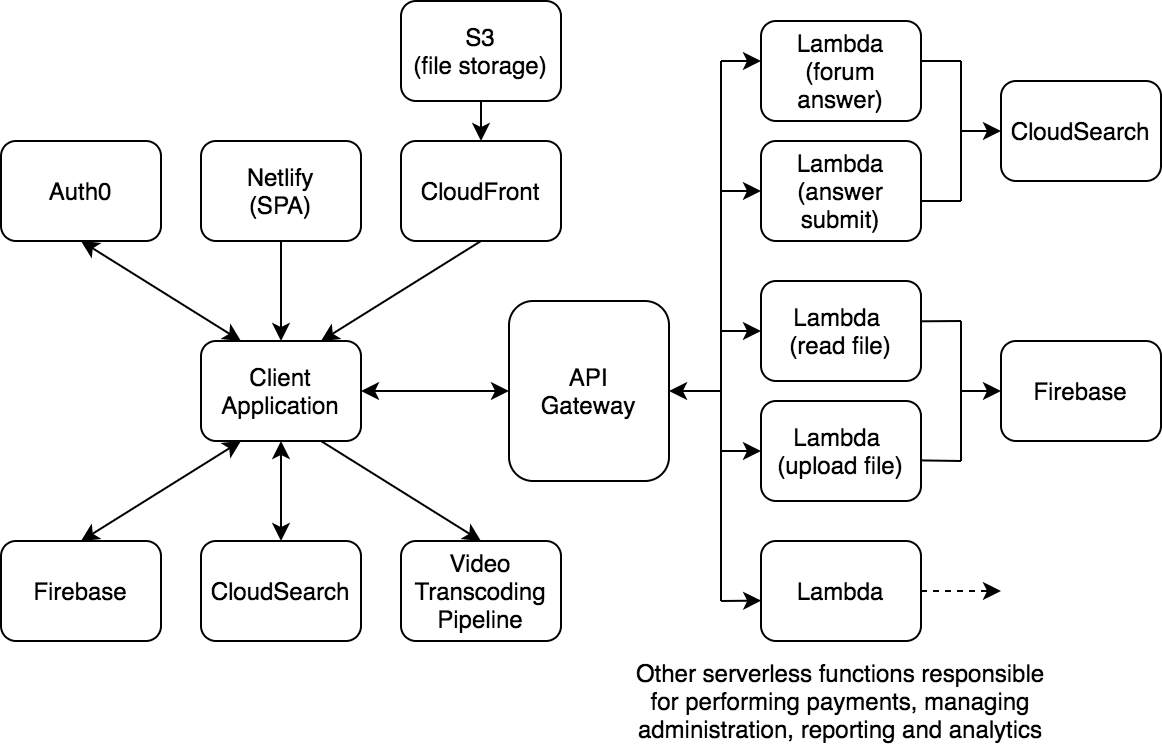
\includegraphics[width=0.8\textwidth]{assets/02-serverless/CloudGuruArchitecture.png}
    \caption{CloudGuru platform architecture}
    \label{fig:cloudguru-architecture-diagram}
\end{figure}

CloudGuru, which is an online educational platform dedicated to people interested in learning numerous cloud related topics, is a good example of such a use-case. Core features of the platform include streaming large selection of video courses, interactive quizzes and practice exams, real-time discussion forum and integrations with third party services enabling users to buy access to the courses.

The architecture of the e-learning platform utilises services of several cloud providers. Frontend of the web application built as a Single Page Application is hosted on Netlify, which acts as a Content Delivery Network (CDN) for the platform client. Auth0 service is responsible for registration and authentication functionalities and provides delegation tokens enabling client application to communicate directly and securely with other services. Firebase is used as a primary database, capable of updating clients in real-time using websockets to push updates to the clients. Questions and answers submitted by users to the forum are persisted in the Firebase, later the data is sent to AWS CloudSearch which is indexing it for further searching, enabling users to find information easier. Instructors can upload videos directly to S3 bucket, which triggers the video transcoding pipeline, which will be discussed in more details in the next section. Users can watch the videos served via CloudFront acting as a CDN if they call the lambda function beforehand giving them the permission to access the video assets for a limited period of time.

\subsection*{Event-driven data processing and manipulation}

% https://livebook.manning.com/book/serverless-architectures-on-aws/chapter-2/36 - CloudGuru

CloudGuru - transcoding videos
MindMup - exporting mindmaps

\cite{MartinFowlerServerless}

one of the standard pattern is media conversion - store file to an S3 bucket taht triggers processing of the stored file

% https://livebook.manning.com/book/serverless-applications-with-node-js/chapter-15/1 -  CodePen, MindMup

\subsection*{Real-time stream processing}

\subsection*{IoT applications}

\subsection*{Webhooks / chat boots / scheduled events}

% Other articles:
% https://jyx.jyu.fi/bitstream/handle/123456789/64836/URN%3ANBN%3Afi%3Ajyu-201906253422.pdf?sequence=1
% https://www.doc.ic.ac.uk/~rbc/papers/fse-serverless-17.pdf
% https://arxiv.org/pdf/1708.08028.pdf